

%\documentclass[3p,times]{elsarticle}

%\usepackage{ecrc} % [headings]{espcrc1}

%\volume{00}

%\firstpage{1}

%\journalname{Procedia Computer Science}

%\jid{procs}

%\jnltitlelogo{Procedia Computer Science}
%\setlength{\parindent}{0pt}
%\setlength{\parskip}{1ex plus 0.5ex minus 0.2ex} 



%\usepackage{color}
%\usepackage{graphicx}
%\usepackage{subfigure}
%\usepackage{placeins}
%\usepackage[font=sf]{caption}
%\usepackage[figuresright]{rotating}


% set the starting page if not 1
% \setcounter{page}{17}

% add words to TeX's hyphenation exception list
%\hyphenation{author another created codependent financial paper re-commend-ed Post-Script}

%-------------------------------------------------------------------------------



%\title{Obsidian: GPU Computing Using Haskell (DRAFT)} 
%\author{Joel Svensson, Koen Claessen and Mary Sheeran} 
%\runauth{Joel Svensson, Koen Claessen and Mary Sheeran}

%% \date{\today} 

% \runtitle{Obsidian: GPU Computing Using Haskell}
%\runauth{Joel Svensson, Koen Claessen and Mary Sheeran}

%\begin{document}
%\begin{frontmatter}

%% Title, authors and addresses

%% use the tnoteref command within \title for footnotes;
%% use the tnotetext command for the associated footnote;
%% use the fnref command within \author or \address for footnotes;
%% use the fntext command for the associated footnote;
%% use the corref command within \author for corresponding author footnotes;
%% use the cortext command for the associated footnote;
%% use the ead command for the email address,
%% and the form \ead[url] for the home page:
%%
%% \title{Title\tnoteref{label1}}
%% \tnotetext[label1]{}
%% \author{Name\corref{cor1}\fnref{label2}}
%% \ead{email address}
%% \ead[url]{home page}
%% \fntext[label2]{}
%% \cortext[cor1]{}
%% \address{Address\fnref{label3}}
%% \fntext[label3]{}

%\dochead{}
%% Use \dochead if there is an article header, e.g. \dochead{Short communication}

%\title{GPGPU Kernel Implementation and Refinement using Obsidian}

%% use optional labels to link authors explicitly to addresses:
%% \author[label1,label2]{<author name>}
%% \address[label1]{<address>}
%% \address[label2]{<address>}

%\author{Joel Svensson}
%\author{Koen Claessen}
%\author{Mary Sheeran}
%\affiliation{Chalmers University of Technology}

%\address{CSE Dept., Chalmers University of Technology, Gothenburg, Sweden} 


\subsection*{Abstract}
Obsidian is a domain specific language for data-parallel programming 
on graphics processors (GPUs). It is embedded in the functional 
programming language Haskell. The user writes code using constructs 
familiar from Haskell (like {\tt map} and {\tt reduce}), recursion 
and some specially designed combinators for combining GPU programs. 
NVIDIA CUDA code is generated from these high level descriptions, and 
passed to the {\tt nvcc} compiler~\cite{CUDAGuide2.0}. Currently, we 
consider only the generation of single kernels, and not their coordination.

This paper is focussed on how the user should work with Obsidian, 
starting with an obviously correct (or well-tested) description of the 
required function, and refining it by the introduction of constructs to 
give finer control of the computation on the GPU. For some combinators, 
this approach results in CUDA code with satisfactory performance, promising 
increased productivity, as the high level descriptions are short and 
uncluttered. But for other combinators, the performance of generated code 
is not yet satisfactory. Ways to tackle this problem and plans to integrate 
Obsidian with another higher-level embedded language for GPU programming in 
Haskell are briefly discussed.




%Obsidian is a domain specific language for Data-parallel 
%programming on graphics processors (GPUs) embedded in Haskell. 
%From high level descriptions, code for execution on a GPU is generated.
%Obsidian generates NVIDIA CUDA code that is passed to the {\tt nvcc} 
%compiler \cite{CUDAGuide2.0}. 

%This paper is mainly focused on the usage of Obsidian. The implementation
%of Obsidian itself and a discussion of how the CUDA code is generated can 
%be found in \cite{JSTECH}.



%\vspace{1pc}
%\end{abstract}

%\begin{keyword}
%% keywords here, in the form: keyword \sep keyword
%Data-parallel \sep Embedded language \sep GPUs \sep Haskell  
%% PACS codes here, in the form: \PACS code \sep code

%% MSC codes here, in the form: \MSC code \sep code
%% or \MSC[2008] code \sep code (2000 is the default)

%\end{keyword}

%\end{frontmatter}


%-------------------------------------------------------------------------------
\subsection{Introduction} 

Multicore and manycore processors are becoming increasingly common. Modern 
graphics processing units (GPUs) are examples of manycore processors. Today 
GPUs come with hundreds of processing elements capable of managing thousands 
of threads \cite{Brief8800}. The Obsidian project is about exploring ways 
to program these new machines.  

Obsidian is a domain specific language for general purpose programming on 
GPUs (GPGPU), capable of generating code for modern NVIDIA GPUs. 
In~\cite{JSMSKC_IFL08} we describe a version of Obsidian that uses a monadic 
interface. In the current version of Obsidian the monad has been replaced 
by another data structure, closely related to Arrows~\cite{Arrows}, representing GPU programs. Although the details are 
left out because of space limitations, the use of this GPU program representation 
can be seen in subsection~\ref{sec:GPUPrograms}. For a description of the implementation 
see~\cite{JSTECH} and for more general information on embedded language 
implementation see~\cite{COMPILEEDSL}.

GPU design is driven by the performance demands of graphics applications. 
The kind of processing that is common in graphics falls in the data-parallel 
category \cite{GEMS2}.
% One example of a computation from graphics is the 
%transformation of vertices between different coordinate systems. That is, 
%each vertex is multiplied by the same transformation matrix, fitting  the 
%data-parallel paradigm perfectly. 



%-------------------------------------------------------------------------------
\subsubsection{NVIDIA GPUs and CUDA}


Starting with the 8000 series of GPUs (the G80 architecture), NVIDIA's 
GPUs came with a unified architecture, meaning that all the 
processing elements on the GPU are of the same kind. This was different from 
the previous generation's GPUs, which typically had two kinds of 
processing elements, fragment and vertex processors.  
%There was one kind of processor designed to process fragment/pixel programs and another to process vertex data. 
Now these two kinds 
of processors are replaced by a single kind with capabilities surpassing both 
of the old ones. This new unified architecture together with development tools 
for GPGPU programming go under the 
name CUDA (Compute Unified Device Architecture) 
\cite{CUDAGuide2.0}. CUDA offers the GPGPU programmer a C %,wwwcuda,Brief8800
compiler and libraries for CUDA enabled GPUs (NVIDIA 8000 series and above).  

Figure~\ref{fig:gpu}, shows a conceptual picture of a CUDA enabled GPU. The GPU 
has a number of {\em Multiprocessors} (MP in the picture). These MPs contain 
a number of small processing elements called {\em Streaming Processors} (SP). 
These SPs operate in an SIMD fashion. All SPs in a given MP execute 
the same instruction each clock cycle. 

Each MP is capable of maintaining a large number of threads in flight at the 
same time. A group of threads running on an MP is referred to as a {\em block}. 
A block can contain more threads then there are processing elements; today a 
block can hold up to 1024 threads. There is a scheduler mapping these threads 
over the SPs available. Threads are scheduled in groups called {\em warps} 
consisting of 32 threads that are executed in an SIMD fashion on the MPs.
Conditionals that take different paths within a warp have a negative effect 
on performance; the two diverging paths will in fact be executed sequentially 
\cite{BestPrac}.
%There are however, more threads in a
%warp then there are SPs, so the SPs are switching threads to work on 
%between every instruction. This means that conditionals that
%take different paths within a warp have a negative effect on performance;
%the two diverging paths will in fact be executed sequentially \cite{BestPrac}. 



The MPs also have local memory that is shared between all the 
SPs of that MP, and thus referred to as {\em Shared Memory} in the figure. 
It can be used to exchange information between threads running 
on the SPs; it can also be used as a software managed cache. 
Threads within a warp can safely communicate using shared memory without 
the need for any synchronisation. Threads from different warps, however, need 
to use a synchronisation primitive to ensure a coherent view of the shared 
memory. In CUDA C this primitive is called {\tt \_\_syncthreads()}. The
{\tt \_\_syncthreads()} primitive provides a barrier that all threads of a 
block must reach before any is allowed to proceed. 

The {\em Global memory} is located off chip and is accessible by all MPs. 
In current GPUs, accesses to this memory are uncached.


\begin{figure}
\begin{center}
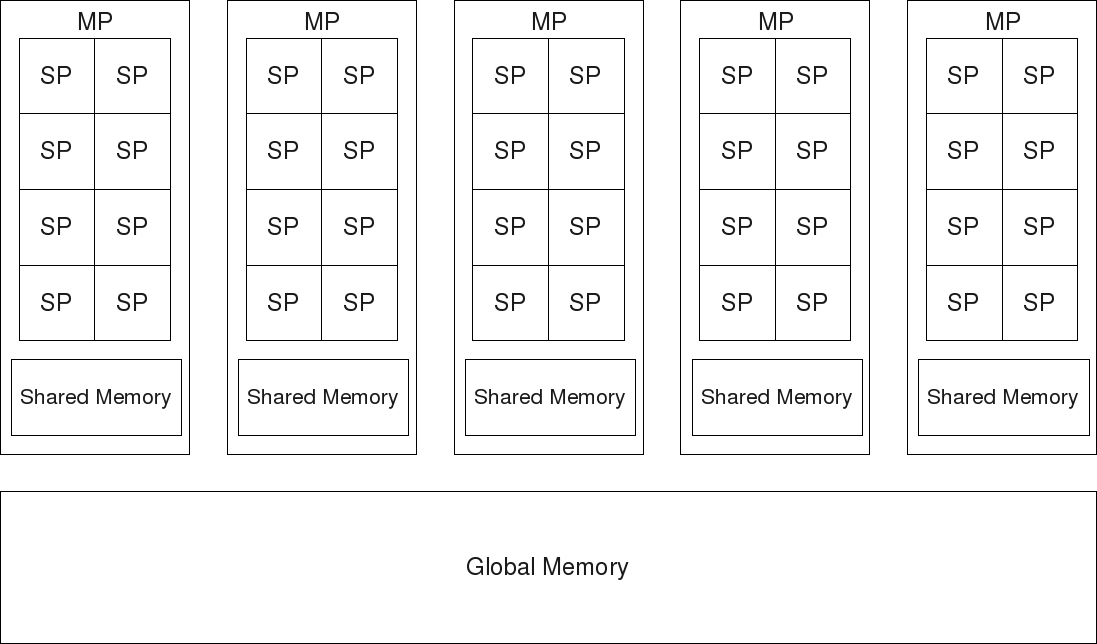
\includegraphics[width=.65\linewidth]{./papp/pictures/gpu.jpg}
\caption{Conceptual image of a CUDA enabled GPU.}
\label{fig:gpu}
\end{center}
\end{figure}

\FloatBarrier

% ------------------------------------------------------------------------------
\subsubsection{Aims of Obsidian}

The initial goal of Obsidian is to simplify the development of GPU kernels, 
the building blocks of larger GPU programs. In the future, ways to combine 
kernels into larger algorithms will also be explored. 

When implementing an algorithm in CUDA, what to compute and how to compute it 
become codependent. Choices such as how many elements the kernel operates on 
and how many threads it uses affect each other greatly. Once a kernel 
is designed with a particular number of elements per thread, this becomes hard to tweak. In CUDA the programmer writes a single program 
parameterised over a thread identity. This program is then executed by 
several threads. Taking this point of view often means that what elements to use 
needs to be computed from the threadIDs. Coming up with these indexing 
computations is not always trivial. 

In Obsidian the program is described as 
a computation between arrays, and combinators are used instead of direct indexing 
into structures. 
Obsidian provides an environment where it is easy to experiment with different
partitionings and choices when implementing an algorithm. It is 
possible to write a simple running first prototype version of a kernel 
without thinking about architectural details. The prototype implementation 
can then be refined into a more efficient implementation. 
The aim of Obsidian is to raise the level of abstraction for the GPGPU 
programmer and to relieve the programmer of details such as laying things out 
in memory. Performance affecting decisions should be easy to make 
and change without major rewrites of the code.



%-------------------------------------------------------------------------------
\subsection{Programming in Obsidian} 

Obsidian is a language for GPGPU programming embedded in Haskell. Many of 
the language features resemble those of Lava, a hardware description and 
verification language \cite{lavaICFP}. The justification to use language 
constructs similar to that of a hardware description language came from 
the observation that GPGPU algorithms often were explained using circuit-like 
pictures, see for example \cite{GEMS3}. 

%Obsidian can be used to describe hardware like algorithms. These are algorithms
%where the number of inputs and outputs are fixed, not dependent on 
%the values of inputs. 
%There are a large number of algorithms falling into this category. For example, 
%there are numerous sorting algorithms (sorting networks) and parallel prefix 
%algorithms implementable in this way. Also, there are examples in the 
%literature where GPGPU programmers implement their kernels to operate on very 
%specific array sizes \cite{GEMS3}. In a later stage, when the kernels are 
%composed into algorithms on large arrays, support for variable length 
%arrays is introduced.

Obsidian can be explained as two sub-languages. First there is a language of 
arrays and operations on arrays, and second, a language that enables mapping of the 
array language programs onto the GPU. 
 
%-------------------------------------------------------------------------------
\subsubsection{Array Language}
\label{sec:ArrayLanguage}
\FloatBarrier
Arrays in Obsidian do not, like in C, name an area of memory. Instead, an 
array is represented by an abstract data type, called {\tt Arr}, supporting 
the following operations: {\tt (!)} for indexing, {\tt len} 
returns the length of an array and {\tt mkArr} that given a function from 
indexes to elements and a length gives an array. For example using these 
operations reversing an array can be accomplished as follows: 

\begin{small}
\begin{verbatim}
rev :: Arr a -> Arr a 
rev arr  = mkArr ixf n
    where 
        ixf ix = arr ! (fromIntegral (n-1) - ix)
        n = len arr 
\end{verbatim}
\end{small}
\noindent
Array reversal is polymorphic in the element type which gives the {\tt rev} 
program the type {\tt Arr a -> Arr a}. 
Internally an array is represented by the computation that gives its elements. 
The array type consists of two parts, a function from indices to elements and an 
integer representing its length:
%-------------------------------------------------------------------------------
\begin{small}
\begin {verbatim} 
data Arr a = Arr (IndexE -> a) Int 
\end{verbatim}
\end{small}
%-------------------------------------------------------------------------------
%An array is a function from an index expression, {\tt IndexE}, to elements.
\noindent 
The length of the array is static, known at compile time, and is represented
by an {\tt Int}. The elements of an array can be {\tt Int}, {\tt Float} or 
{\tt Bool} valued expressions, represented by the types {\tt IntE}, 
{\tt FloatE} and {\tt BoolE}. Arrays can also contain arrays and tuples 
as elements. 

Obsidian provides a number of functions on this array type. For example, 
a function can be mapped over an array using {\tt fmap}. 
%see figure~\ref{fig:zipunzip}:

%-------------------------------------------------------------------------------
\begin{small}
\begin{verbatim}
fmap :: (a -> b) -> Arr a -> Arr b
\end{verbatim}
\end{small}
%-------------------------------------------------------------------------------
\noindent
The array type is also an instance of {\tt Foldable}, so there is a function 
{\tt foldr} (often called {\tt reduce}) defined on arrays: 

\begin{small}
\begin{verbatim}
foldr :: (a -> b -> b) -> b -> Arr a -> b
\end{verbatim}
\end{small}
\noindent
Two other basic functions on arrays that are available are {\tt pair} and 
{\tt unpair}: 
\begin{small}
\begin{verbatim}
pair :: Arr a -> Arr (a,a)
unpair  :: Choice a => Arr (a,a) -> Arr a
\end{verbatim}
\end{small}
\noindent
The function {\tt pair} takes an array and returns an array of pairs where 
the first element of the input array is paired up with the second, the 
third with the forth and so on. The {\tt unpair} function does the 
opposite. % see figure~\ref{fig:pairunpair}.

The {\tt Choice} class contains those types that have an {\tt ifThenElse} 
function defined on them:  
\begin{small}
\begin{verbatim}
ifThenElse :: Choice a => BoolE -> a -> a -> a
\end{verbatim}
\end{small}
\noindent
Another example of a function given in the array library is {\tt zipp} of type{\tt (Arr a, Arr b) -> Arr (a, b)}.
%\begin{small}
%\begin{verbatim}
%zipp :: (Arr a, Arr b) -> Arr (a, b)
%\end{verbatim}
%\end{small}
This function performs on arrays what the normal Haskell {\tt zip} 
does on lists. However, the input to {\tt zipp} is a pair of arrays. 

%Array programs like those described here make up the building blocks used
%to form larger GPU programs. How to create a GPU program from these is 
%shown in the following subsection. 


%-------------------------------------------------------------------------------

%\FloatBarrier
\subsubsection{GPU Programs}
\label{sec:GPUPrograms}

The second layer of Obsidian offers a data type that represents a GPU program
with input {\tt a} and output {\tt b}:

\begin{small}
\begin{verbatim} 
data a :-> b = ... 
\end{verbatim}
\end{small} 
\noindent
%The details of {\tt a :-> b} are shown in subsection~\ref{sec:Implementation}. 
\noindent
Informally we can think of {\tt a\nolinebreak~:->\nolinebreak~b} as representing programs that operate 
as illustrated in figure~\ref{fig:program}. This figure 
shows a program that performs some computation using a number of threads 
followed by a barrier synchronisation, and so on. The contents of the 
boxes marked with {\em Pure} can be thought of as containing an array 
program.% such as those in subsection~\ref{sec:ArrayLanguage}.
The type constructor {\tt :->} is a variant of an arrow, which in turn is a generalisation of a monad~\cite{JSTECH}.
%
\begin{figure}
\begin{center}
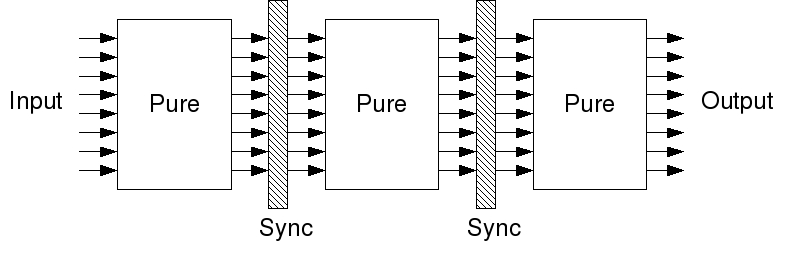
\includegraphics[width=.60\linewidth]{./papp/pictures/prg_intuit.jpg}
\caption{A GPU program of type  {\tt a :-> b} can be thought 
of as pure computations interspersed by syncs.}
\label{fig:program}
\end{center}
\end{figure}
\noindent
One way to create a GPU program is by using the function {\tt pure} of type {\tt (a -> b) -> a :-> b}.
%\begin{small}
%\begin{verbatim}
%pure :: (a -> b) -> a :-> b
%\end{verbatim}
%\end{small}
For example the array language program {\tt fmap (+1)}, that increments 
every element of an array, can be lifted to a GPU program: 
%
\begin{small}
\begin{verbatim}
incr :: Arr IntE :-> Arr IntE 
incr = pure $ fmap (+1)
\end{verbatim}
\end{small} 
 \noindent
GPU programs can be executed on the GPU from
{\em GHCi} (the Haskell interpreter) using the function {\tt execute}: 

\begin{small}
\begin{verbatim}
execute :: (Flatten a, Flatten b) 
         => (Arr a :-> Arr b) -> [a] -> IO [b]
\end{verbatim}
\end{small}
\noindent
%The class {\tt Flatten} will be explained in detail in 
%subsection~\ref{sec:Implementation}, but 
Instances of {\tt Flatten} are all the types that can be stored in the 
GPU memory. Examples of types that are in {\tt Flatten} are {\tt IntE}, 
{\tt FloatE}, {\tt BoolE}. Arrays and pairs of things that are in Flatten 
are also instances of {\tt Flatten}.
Here, {\tt execute} is used in order to run an instance of the {\tt incr} 
program on the GPU:

\begin{small}
\begin{verbatim}
*Obsidian> execute incr [0..9]
[1,2,3,4,5,6,7,8,9,10]
\end{verbatim}
\end{small}
\noindent
The elements of the Haskell list given to {\tt execute} are used to create 
an input array to the kernel. Following this, the kernel is executed on the
GPU and the result is read back and presented as a Haskell list. 

In the example above, the {\tt execute} function generates the following kernel 
corresponding to the given GPU program:
\begin{small}
\begin{verbatim}
__global__ void generated(word* input,word* result){
  unsigned int tid = (unsigned int)threadIdx.x;
  extern __shared__ unsigned int s_data[];
  word __attribute__((unused)) *sm1 = &s_data[0];
  word __attribute__((unused)) *sm2 = &s_data[0];
  ix_int(result,tid) = (ix_int(input,tid) + 1);
}
\end{verbatim}
\end{small}
\noindent
The generated kernel has two arguments, an input array of words and an 
output array of words. Words represent 32-bit quantities that can be either
floating point or integer valued. This particular kernel does not use 
any shared memory; the incremented values are stored directly into the 
result array that resides in global memory.  

Given two GPU programs, {\tt f} and {\tt g}, of suitable types, a 
composite GPU program can be created by passing the output of {\tt f} to the 
input of {\tt g}. In Obsidian this is done using the composition operator (or combinator)
{\tt (->-)}: 


\begin{small}
\begin{verbatim}
(->-) :: (a :-> b) -> (b :-> c) -> (a :-> c)
\end{verbatim}
\end{small}
\noindent
The following illustrates the use of {\tt (->-)} by implementing a 
program that increments every element of an array but also reverses 
the array: 

\begin{small}
\begin{verbatim}
increv :: Arr IntE :-> Arr IntE 
increv = pure (fmap (+1)) ->- pure rev

*Obsidian> execute increv [0..9]
[10,9,8,7,6,5,4,3,2,1]
\end{verbatim}
\end{small}
\noindent
The code generated from the {\tt increv} program is very similar to that 
of {\tt inc} but the indexing is reversed:

\begin{small}
\begin{verbatim}
__global__ void generated(word* input,word* result){
  unsigned int tid = (unsigned int)threadIdx.x;
  extern __shared__ unsigned int s_data[];
  word __attribute__((unused)) *sm1 = &s_data[0];
  word __attribute__((unused)) *sm2 = &s_data[0];
  ix_int(result,tid) = (ix_int(input,(9 - tid)) + 1);
}
\end{verbatim}
\end{small}
\noindent
The code generated for the {\tt incr} and {\tt increv} examples uses 
$10$ threads to compute the resulting array. By default, the result will 
be computed using a number of threads equal to the number of elements in 
the return array. 

The {\tt increv} program can also be specified with an explicit storing 
of intermediate values between the {\tt rev} and the {\tt fmap (+1)}. 
This is accomplished using a primitive GPU program called {\tt sync}:

\begin{small}
\begin{verbatim}
sync  :: Flatten a => Arr a :-> Arr a

increv :: Arr IntE :-> Arr IntE 
increv = pure (fmap (+1)) ->- sync ->- pure rev
\end{verbatim}
\end{small} 
\noindent
This version of {\tt increv} computes the same result as the previous one. 
However, it does so by computing {\tt fmap (+1)} on the array, storing the
intermediate result in shared memory followed by computing the reverse.
The CUDA C code for this version of {\tt increv} looks like this. Notice 
how the shared memory is used and the call to {\tt \_\_syncthreads()}: 
%
\begin{small}
\begin{verbatim}
__global__ void generated(word* input,word* result){
  unsigned int tid = (unsigned int)threadIdx.x;
  extern __shared__ unsigned int s_data[];
  word __attribute__((unused)) *sm1 = &s_data[0];
  word __attribute__((unused)) *sm2 = &s_data[8];
  ix_int(sm1,tid) = (ix_int(input,tid) + 1);
  __syncthreads();
  ix_int(result,tid) = ix_int(sm1,(7 - tid));
}
\end{verbatim}
\end{small}


\subsection{Outline of Code Generation}
\label{sec:CodeGen}
\FloatBarrier

This subsection briefly reviews the code generation process using 
a hyphothetical program as example. The program under consideration 
is this: 

\begin{small}
\begin{verbatim}
prg = pure (fmap f) ->- sync -> rev ->- sync ->- pure (fmap g) 
\end{verbatim}
\end{small}

This program applies some function {\tt f} to all elements of 
an array. The array is then reversed and lastly a function {\tt g} 
is applied to all elements. Between every operation there is a {\tt sync}.
The program {\tt prg} is an element of the datatype {\tt (a :-> b)}. 
To see what happens during code generation, it is necessary to know 
the implementation of this type.
\begin{small}
\begin{verbatim} 
data a :-> b 
   = Pure (a -> b) 
   | Sync (a -> Arr FData) (Arr FData :-> b) 
\end{verbatim}
\end{small} 
\noindent
The type {\tt (a :-> b)} is essentially a list of computations. The 
function {\tt pure} is directly implemented using the constructor 
{\tt Pure}. The function {\tt sync} is implemented in terms of the 
constructor {\tt Sync}:

\begin{small}
\begin{verbatim} 
sync :: Flatten a => (Arr a :-> Arr a)
sync = Sync (fmap toFData) (pure (fmap fromFData))
\end{verbatim}
\end{small} 
\noindent
The example program {\tt prg} would be represented as follows: 
%
\begin{small}
\begin{verbatim} 
Sync (fmap (toFData . f)) 
     (Sync ((fmap toFData) . rev . (fmap fromFData)) 
           (Pure (fmap g)))   
\end{verbatim}
\end{small} 
\noindent
From this representation, which is essentially the list {\tt [fmap f, rev, fmap g]},
the CUDA code is generated as outlined in figure~\ref{fig:codegen}. 
An input array is created and applied to the first stage of the computation, 
{\tt (fmap f)}, resulting in: 
\begin{small}
\begin{verbatim}
Arr (\ix -> f(index (variable ``input'') ix)) n. 
\end{verbatim}
\end{small}

The information given by this array is used to construct the C assignment 
statement {\tt sm1[tid] = f(input[tid])} as seen in the figure.

Following this a new Obsidian level array that indexed into {\tt sm1} is 
created and used as input to the second stage of the computation. 

%Following this a new Obsidian level array that looks as follows is created: 
%\begin{small}
%\begin{verbatim}
%Arr (\ix -> index (variable ``sm1'') ix) n. 
%\end{verbatim}
%\end{small}



%This expression is used to generate a 
%C assignment. The array is stored into one of two shared memory arrays 
%This array  is used as input to the next phase. The computation is then double 
%buffered between the two shared memory arrays. 
%giving an expression.


\begin{figure}
\begin{center}
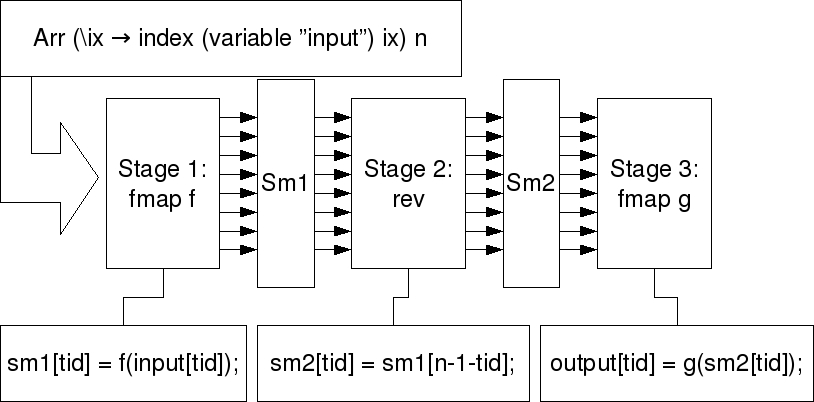
\includegraphics[width=.65\linewidth]{./papp/pictures/codegenexample.jpg}
\caption{Outline of the code generation procedure.}
\label{fig:codegen}
\end{center}
\end{figure}


%-------------------------------------------------------------------------------

\subsection{Case Studies}
\label{sec:CaseStudies}

\FloatBarrier
This subsection describes a few slightly larger Obsidian programs. The main purpose of this subsection is to show 
how we want to write GPGPU programs using Obsidian. 
%How the performance 
%of the generated code can be improved is discussed in subsection~\ref{sec:FutureWork}  
%%% Move this later.  XXX

\subsubsection{Sorting}

Sorting is a popular function to place on the GPU, see~\cite{SINTORNSORT,SORT3}.
{\em Odd-Even merge sort}, due to Batcher, uses a merger component called the Odd-Even merger. This 
merger merges two sorted arrays. In Obsidian this merger and sorter 
can be implemented using the combinators {\tt two}, {\tt ilv}, {\tt evens}
and {\tt odds}. For a detailed description of these combinators see
~\cite{LAVASORTER}.

\begin{small}
\begin{verbatim}
mergeOE :: (Choice a, Flatten a) 
         => Int -> ((a,a) -> (a,a)) -> (Arr a :-> Arr a)
mergeOE 1 f = pure (evens f)
mergeOE n f = ilv (mergeOE (n-1) f) ->- sync ->- pure (odds f)
\end{verbatim}
\end{small}
\noindent
This is actually a pattern into which any two-input two-output function
can be plugged. However, we choose the following {\em comparator} function (a compare and swap operation). The resulting merger can be executed on the GPU.
\begin{small}
\begin{verbatim}
cmp :: (Ordered a, Choice (a, a)) => (a, a) -> (a, a)
cmp (a,b) = ifThenElse (a <* b)  (a,b) (b,a)

*Obsidian> let input = ([1,3,5,7,2,4,6,8] :: [IntE]) 
*Obsidian> execute GPU (mergeOE 3 cmp) input
[1,2,3,4,5,6,7,8]
\end{verbatim}
\end{small}
\noindent
Given this merger, the sorter is implemented by recursively sorting 
two halves of the input array followed by an application of the merger:

\begin{small}
\begin{verbatim}
sortOE :: Int -> (Arr IntE :-> Arr IntE)
sortOE  0 =  pure id
sortOE  n =  two (sortOE (n-1)) ->- sync ->- mergeOE n cmp 

*Obsidian> execute GPU (sortOE 3) [6,0,1,3,4,2,5,7]
[0,1,2,3,4,5,6,7]
\end{verbatim}
\end{small}

The performance of the code generated from this sorter specification is poor. It
runs about three times slower than the example Bitonic
sorter distributed with the CUDA SDK. 
The reason is that nested applications of the {\tt two} and {\tt ilv} 
combinators are hard to optimise. We expect that single (parameterised) combinators corresponding
to particular nestings of these combinators will bring significant performance improvement.
%
%The reason for the poor performance in this case is the code 
%condition of the code generated from the deep nestling of applications of 
%{\tt two} and {\tt ilv} that the code generator currently does a very bad job 
%at optimising. There may be alternative ways to implement these combinators 
%or entirely different ones should replace them. 


%-------------------------------------------------------------------------------
\subsubsection{Parallel Prefix}
\FloatBarrier

This subsection shows the implementation of a parallel prefix (also called scan) 
kernel, known as {\tt sklansky} after J. Sklansky \cite{Sklansky}.
This kernel will then be optimised step-by-step using Obsidian. This 
optimisation effort uses an experimental feature of Obsidian called {\tt syncHow}. 
This is different from the normal {\tt sync} in the way it assigns work to threads. 
For a more thorough explanation of {\tt syncHow} see ~\cite{JSTECH}.
For an explanation of the parallel-prefix operation see~\cite{BlellochTR90}. 

The sklansky parallel prefix algorithm 
is implemented by splitting the inputs in two halves and recursively 
applying sklansky to both halves. The two sub-results are then 
joined by applying the operation between the highest index of the first
sub-result and all the elements in the second sub-result, this is done 
using a function called {\tt fan}: 

\begin{small}
\begin{verbatim}
fan op arr = conc (a1, (fmap (op c) a2)) 
    where (a1,a2) = halve arr
          c       = a1 ! (fromIntegral (len a1 - 1))
\end{verbatim}
\end{small}
\noindent
The {\tt sklansky} function is now implemented using 
{\tt two} and {\tt fan}: 

\begin{small}
\begin{verbatim}
sklansky :: (Flatten a, Choice a) 
          => Int -> (a -> a -> a) -> (Arr a :-> Arr a) 
sklansky 0 op = pure id
sklansky n op = two (sklansky (n-1) op) ->- 
                pure (fan op) ->- sync
\end{verbatim}
\end{small}

Executing ({\tt sklansky 3 (+)}) on the GPU given input {\tt [0..7]} computes
the prefix sum as expected, returning {\tt [0,1,3,6,10,15,21,28]} 
%Executing a small instance of the prefix network above on the GPU has 
%the following result: 

%\begin{small}
%\begin{verbatim}
%*Obsidian> execute (sklansky 3 (+)) ([0..7] :: [IntE])
%[0,1,3,6,10,15,21,28]
%\end{verbatim}
%\end{small}

If {\tt sklansky} is used to generate code for an array of 512 elements,
it uses 512 threads to calculate the prefix sums. However, the number of 
applications of the {\tt op} operator that is needed in any stage of the 
algorithm is only 256. This indicates that 
using 256 threads to compute the result would give more efficient
use of the GPU's resources.

Since the code generated by Obsidian is not by default {\em in-place} with regard 
to shared memory, each thread in the 256 threaded program needs to both perform 
the operation between two elements and copy one value unchanged. This is desired
because then each thread performs the exact same operations,
which means that there is no risk for divergence within a warp. 

This perfect division of labour is not obtainable with the current 
implementation of the {\tt How} argument to {\tt sync}. However, one 
division of the work that has experimentally been shown to perform well, see 
table in next subsection,  
is to let each thread $tid$ perform the work of $tid$ and $tid + 256$. This 
program is shown below: 

\begin{small}
\begin{verbatim}
sklansky1 :: (Flatten a, Choice a) 
           => Int -> (a -> a -> a) -> (Arr a :-> Arr a) 
sklansky1 0 op = pure id
sklansky1 n op = two (sklansky1 (n-1) op) ->- 
                 pure (fan op) ->- syncHow (pairNth 256) 
\end{verbatim}
\end{small}


Another optimisation to apply to the sklansky algorithm is the removal of 
unnecessary {\tt \_\_syncthreads()} calls from the generated code, this is 
done by using {\tt syncWarp}. It is up to the programmer to ensure that it 
is safe to use {\tt syncWarp}. For a sklansky network of size 32, it should 
be safe to leave out the {\tt \_\_syncthreads} since all of the communication 
stays within a warp. Using this information leads to the following code where 
the sklansky networks of size 32 or smaller use {\tt syncWarpHow}.


\begin{small}
\begin{verbatim} 
sklansky2 :: (Flatten a, Choice a) 
           => Int -> (a -> a -> a) -> (Arr a :-> Arr a) 
sklansky2 0 op = pure id
sklansky2 n op = two (sklansky2 (n-1) op) ->- pure (fan op) 
                   ->-  if n <= 5 
                         then syncWarpHow (pairNth 256)
                         else syncHow (pairNth 256)
\end{verbatim}
\end{small}

%% XXX Why is there no explicit 32 anywhere in the vicinity of SyncWarpHow?

A last tweak to force the algorithm to compute {\em in-place}. This 
is accomplished using the primitives {\tt syncIP} and {\tt syncIPHow}, which
are variants of {\tt sync} that enforce {\em in-place} computation.

%-------------------------------------------------------------------------------
\subsubsection{Parallel Prefix Sums on large arrays}
\FloatBarrier

The Sklansky kernels given above can be used in an algorithm that computes 
the parallel prefix of a large array. This is done in the same way as in
~\cite{ScanCUDA}.
The table below shows the results of using the different parallel prefix 
kernels from above in an algorithm for computing the prefix sums of 
$2^{20}$ elements.

\begin{small}
\begin{center}
  \begin{tabular}{  l | r | r |r | r  }
    %\hline
    Kernel          & In-place & Sync in Warp & Threads & ms   \\ \hline
    NVIDIA SDK      & Yes      & N/A          & 256     & 0.64 \\
    Hand Optimised  & Yes      & No           & 256     & 0.74 \\ 
    sklansky        & No       & yes          & 512     & 1.06 \\ 
    sklansky1       & No       & yes          & 256     & 0.89 \\ 
    sklansky2       & No       & No           & 256     & 0.86 \\ 
    sklansky3       & Yes      & No           & 256     & 0.79 \\
    %\hline
  \end{tabular}
\end{center}
\end{small}

The table above shows the running times of six different Sklansky kernels. 
All runtime measurements where performed on an NVIDIA 9800GX2 using one GPU. 
The code labeled {\em Hand Optimised} was written directly in CUDA. 
This kernel was the result of two afternoons of optimisation effort by 
two people. The three following kernels {\em sklansky} to {\em sklansky2} are 
generated from the given Obsidian programs. The version called {\em sklansky3} 
is identical to {\tt sklansky2} except is in-place. Even the very first version, 
{\em sklansky} performs reasonably well, but by using the experimental features 
the performance can be pushed quite close to the hand optimised version.  
The fastest kernel, called {\em NVIDIA SDK}, is the one supplied 
with the CUDA SDK. This kernel is based on the Brent-Kung network and its 
implementation is shown in~\cite{ScanCUDA}. The {\tt NVIDIA SDK} 
kernel is highly optimized with regards to its memory access pattern and 
so the code is considerably more complicated than that of any of the Obsidian parallel-prefix kernels.
 

%-------------------------------------------------------------------------------
\FloatBarrier
\subsection{Future work}
% \label{sec:PAPPFutureWork}

Obsidian is work in progress and as such it changes a lot. Future work will both
explore improvements to code generation for kernels and ways to coordinate kernels.

In order to get to the quite efficient version of the {\tt sklansky} kernel 
in subsection~\ref{sec:CaseStudies}, the experimental {\tt How} argument to {\tt sync} was needed. 
This needs to be 
explored further. {\tt How} as it is today, any function of type
{\tt IndexE -> [IndexE]}, offers too much freedom and with that the risk of
introducing errors. We are searching for an elegant model for expressing how and what 
to compute, and for ways to integrate this with
the language. This is our biggest research challenge.

Subsection~\ref{sec:CaseStudies}, on case studies, showed that it is possible to
generate quite efficient code from Obsidian programs. The current version 
generates efficient code for very specific uses of the {\tt two} combinator, 
for example the kind used in the {\tt sklansky} parallel prefix network. More 
work needs to be done in order to find a good way to produce efficient code 
for a larger set of combinators. 
This may very well involve designing new combinators that do not need
to be nested as the current ones do.

The CUDA code generated by Obsidian uses very few registers. In fact,
the generated code is under-utilizing the resources of the GPU. The generated 
code also contains many common subexpressions. This hints that applying a 
step of common subexpression elimintaion would be beneficial, increasing 
the register use and reducing the repeated computation of values. Performing
common subexpression elimination would also lower the instruction count,
which is quite high to begin with, because loops are unrolled. 
The register usage and instruction count values on which these conclusions 
are based where obtained using the CUDA profiler supplied as part of the 
CUDA toolkit~\cite{wwwcuda}.

Obsidian can currently only be used to generate kernels, the small 
building blocks used to form larger GPU algorithms. As future work, 
methods of describing kernel coordination in a high level fashion will 
be investigated.

At the University of New South Wales, Manuel Chakravarty 
et. al. are developing another language for GPGPU programming
called Accelerate. Accelerate is also embedded in Haskell, but intends
to be at a higher 
level of abstraction than Obsidian. Accelerate supplies the programmer 
with a collection of basic building blocks for data parallel programming. 
Amongst these building blocks are {\tt map}, {\tt zipWith} and {\tt scan}.
With the Accelerate team at UNSW, we are looking into 
ways of combining the two complementary approaches. In this setting Obsidian 
could be used to generate the underlying kernels (the building blocks) that the Accelerate 
programmer uses to build a GPGPU application. 

A limitation of Obsidian is the inability to express algorithms where 
the length of the output array is dependent on the input data. 
An example of such a data dependent algorithm is {\tt filter}. The {\tt filter} 
function takes a sequence of elements and a predicate and produces a sequence 
of those elements for whom the predicate holds. Future work 
will also consist of searching for a suitable minimal language construct
to add that enables expressing such algorithms. 






%-------------------------------------------------------------------------------
\subsection{Related work}

GPUs are becoming more and more interesting to use in non-graphical applications.
A modern GPU is a manycore machine with, today, hundreds of processing elements. 
The question of how to program these machines arises. NVIDIA's answer is CUDA
\cite{CUDAGuide2.0}. CUDA supplies a slightly extended version of C in which 
the programmer can specify GPU kernels and the controlling CPU program in the 
same language. In CUDA the programmer writes a single program parameterised 
over a thread identity. Compare this to Obsidian where the program describes 
a computation over an array. 

There are a number of other C/C++ based languages that target 
GPGPU programmers, for example Brook\cite{Brook} and 
RapidMind\cite{RapidMind}. Brook, CUDA and RapidMind are major improvements from 
what was previously available for the programmer interested in general purpose 
computations on the GPU. 
%Before these, the GPGPU programmer only had the 
%graphics API to work with and needed to translate his or her programs into 
%graphics vocabulary in order to use the GPU. 

Higher level approaches are also being investigated. PyGPU embedds a GPGPU 
programming language in Python\cite{PyGPU}. PyGPU makes use of Python's 
introspective abilities to generate efficient code. 

Like Obsidian, Accelerate is embedded in Haskell \cite{GPUGEN}. Accelerate 
however, is higher level language than Obsidian. Where the purpose of 
Obsidian is to implement basic algorithmic building blocks such as 
reductions and prefix sums, Accelerate provide these building blocks as 
primitives. 

Vertigo is another GPU programming language embedded in Haskell\cite{VERTIGO}.
Vertigo can be used to describe procedureal surfaces and textures and generates
efficient DirectX9 shader code. 

There are also many examples of domain specific languages (DSLs)
that target not only GPUs but also other platforms, such as multicore machines.
Of particular interest to us is Microsoft's Accelerator project~\cite{ACCELERATOR}. Interestingly, Accelerator includes the same restriction to ``hardware-like'' algorithms as Obsidian does.
%However, Vertigo is targeting graphical applications. 

%There are also many examples of languages that do not specifically target 
%GPUs but experiment with new methods and ways of parallel programming. 
%In this category we have Sequoia, where the memory hierarchy is in focus. 
%Sequoia programs can for example be compiled to the Cell BE architecture. 
%Data-Parallel Haskell extends Haskell with parallel arrays and operations 
%on parallel arrays\cite{DPH}. Data-Parallel Haskell implements the nested 
%data-parallel paradigm and is in that sense following in the path of 
%NESL\cite{NESL}. 


 



%\begin{itemize}
%\item Chapel \cite{Chapel}
%\item DPH \cite{DPH}
%\item Fortress \cite{fortress}
%\item GPUGen \cite{GPUGEN}
%\item Lava \cite{lavaTutorial}
%\item RapidMind \cite{RapidMind}
%\item Sequoia \cite{SEQUOIA}
%\item X10 \cite{X10}
%\end{itemize}

\subsection{Discussion and conclusion}

Obsidian is work in progress and there are many loose ends to tie up and 
paths left to explore. In subsection~\ref{sec:CaseStudies}, the 
strengths of Obsidian show; it is possible to express quite complex algorithms
using short and elegant programs. The case studies also show that it is possible
to generate quite efficient code from these high level descriptions. However, 
this needs more work in order to more reliably produce efficient code and
to broaden the available set of combinators for combining GPU programs.

%Another benefit of a higher level language such as Obsidian compared to 
%CUDA is the ability to reuse code. There is an example of this too in the 
%case studies subsection where a single reduction program can be used to generate
%code to compute the maximum, minimum and sum very easily. 

%Compositionally, or the ability to use already written programs as building
%blocks in other programs is another area where Obsidian is an improvement 
%over working in languages such as C for GPU programming. If in CUDA you have
%one Kernel that computes the 
 
%In Obsidian it is easy to describe an initial prototype solution to a problem,
%such as for example the {\tt mySum} kernels in subsection~\ref{sec:SyncPar}. 
%It requires no deep knowledge of the GPU architecture but works out of the 
%box. The prototype implementation can be tweaked into a more efficient 
%implementation by performing small changes to the Obsidian code that often 
%lead to quite large differences in the generated C code. An example of this 
%is {\tt mySum1} against {\tt mySum2} where adding a single {\tt sync} leads 
%to a radically different C program. 


 

Obsidian offers the GPGPU programmer a higher level language, while trying 
not to sacrifice too much performance. When Programming in CUDA C, the indexing
arithmetic often gets quite complex. This is a common trait of data-parallel 
programming in C-like languages. One goal of Obsidian is to be able to express 
these algorithms without the complex index manipulations; instead the data 
access pattern is captured in the use of functions such as {\tt pair} and 
{\tt two} or in the recursive structure of the Obsidian program. 


%Obsidian is also an improvement over CUDA in the area of code reuse. The 
%{\tt reduce} function from subsection~\ref{sec:CaseStudies} is an example of this. 
%Obsidian is also compositional in another way than CUDA. Reusing kernels as
%building blocks in other kernels is in CUDA not realistic, while in Obsidian 
%it is the preferred way to write programs. Take as an example of this the 
%mergers and sorters in subsection~\ref{sec:CaseStudies}. In CUDA you would design 
%one kernel from scratch implementing the merger and sorter simultaneously. 

This paper presented Obsidian an embedded language for GPGPU programming that
offers a higher level of abstraction compared to languages such as CUDA. 
Obsidian allows the programmer to think more of the algorithm and less of 
architectural details of the GPU. The contributions of Obsidian to the GPGPU 
field is a higher level programming environment that eases experimentation. 

\subsection*{Acknowledgments}
\noindent
This research is funded by the Swedish Research Council.

%-------------------------------------------------------------------------------

%-------------------------------------------------------------------------------


%\bibliographystyle{elsarticle-num}
%\bibliography{obs_okt}
		




%\begin{figure}
%\centering
%\begin{minipage}{.5\linewidth}
%  \centering
%  \includegraphics[width=.9\linewidth]{./Pictures/sklansky-g1}
%  \caption{Stage 1}
%  \label{fig:fig_G1}
%\end{minipage}%
%\begin{minipage}{.5\linewidth}
%  \centering
%  \includegraphics[width=.9\linewidth]{./Pictures/sklansky-g2}
%  \caption{\small{Stage 2}}
%  \label{fig:fig_G2}
%\end{minipage}
%\end{figure}


%\end{document}
